\section{Conditional Wilson inequalities and a score criterion}\label{cl:sec:fisher}

The trace identity of Section~\ref{cl:sec:replica} requires a bound under
squared-likelihood tilted histories. We first prove a conditional
inequality for the actual Wilson vacuum, without a restriction to calm
fields, and then use it to obtain a sufficient score estimate for the
cube datum. The conditional inequality is uniform in volume. The score
estimate still requires control across a physical time interval.

\subsection{Every one-link conditional vacuum law}
Let $s$ be a three-dimensional spatial torus whose sides are at least three,
and let $b=\beta_W\ge0$. Use the exact $\SU(2)$ transfer kernel
\eqref{cl:eq:kernel-A}, with
\[
S_{\rm sp}(Q)=\frac b2\sum_{p\text{ spatial}}\ReTr Q_p,
\qquad D_b(Q)=e^{S_{\rm sp}(Q)/2}.
\]
Let $h_b>0$ be its unit Perron eigenfunction and
$\pi_b(dQ)=h_b(Q)^2dQ$. Order the spatial links arbitrarily. A prefix
history fixes an initial segment of this order; all later links remain
integrated over. Each $\SU(2)$ factor in this section has the unit-round
$S^3$ metric.\footnote{This metric convention applies to the gradients in
this section. The metric $-\Tr(XY)$ used for curvature earlier in the
paper is twice the unit-round metric on $\SU(2)$. A constant rescaling
of the metric rescales both the Poincar\'e constant and the squared
gradient inversely, leaving their product unchanged.}

\begin{theorem}[conditional vacuum comparison]\label{cl:thm:link-poincare}
For every finite $b\ge0$, every link ordering and every prefix history,
the conditional density $\rho_j$ of the next link relative to probability
Haar measure obeys
\begin{equation}\label{cl:eq:prefix-density}
\frac{\rho_j(u)}{\rho_j(v)}\le e^{12b}
\qquad(u,v\in\SU(2)).
\end{equation}
Consequently every smooth real $f$ on that link satisfies
\begin{equation}\label{cl:eq:prefix-poincare}
\operatorname{Var}_{\pi_{b,j}}(f)
\le \frac{e^{12b}}3\int |\nabla f|^2\,d\pi_{b,j}.
\end{equation}
The constants are independent of spatial volume and the prefix history.
\end{theorem}
\begin{proof}
Suppose $Q,\widetilde Q$ differ on one spatial link. That link belongs
to four spatial plaquettes. Each contribution $(b/2)\ReTr Q_p$ lies in
$[-b,b]$, hence
\[
|S_{\rm sp}(Q)-S_{\rm sp}(\widetilde Q)|\le8b.
\]
For fixed $Q'$ and temporal links, exactly one term in the temporal
action contains the changed bottom link. Its change is at most $2b$.
Comparison before the temporal Haar integration therefore gives
\[
e^{-2b}\le\frac{A_b(Q,Q')}{A_b(\widetilde Q,Q')}\le e^{2b}.
\]
Put $g_b=h_b/D_b$. The Perron equation reads
\[
\lambda_b g_b(Q)=\int A_b(Q,Q')D_b(Q')h_b(Q')\,dQ'.
\]
Its integrand, apart from $A_b$, has a positive weight independent of $Q$.
Thus $g_b(Q)/g_b(\widetilde Q)$ lies in $[e^{-2b},e^{2b}]$.
As $h_b^2=e^{S_{\rm sp}}g_b^2$, we obtain
\begin{equation}\label{cl:eq:vacuum-local-ratio}
e^{-12b}\le\frac{h_b(Q)^2}{h_b(\widetilde Q)^2}\le e^{12b}.
\end{equation}
Fix any prefix, replace the next link $u$ by $v$, and integrate all
unrevealed links with product Haar measure. The same bounds hold pointwise
before integration, and hence after integration. Normalising the
conditional law cancels in the density ratio. This proves
\eqref{cl:eq:prefix-density} for every history. All densities are smooth
and positive: the kernel is smooth and positive on a compact space, and
the Perron equation preserves smoothness.

On the unit round $S^3$, Haar measure has Poincar\'e constant $1/3$.
Indeed the eigenvalues of $-\Delta_{S^3}$ on restrictions of homogeneous
harmonic polynomials of degree $r$ are $r(r+2)$. This follows by writing
the Euclidean Laplacian in polar coordinates and applying it to
$R^rY(\omega)$. Harmonic decomposition of polynomials and density of their
restrictions in $L^2(S^3)$ give a complete orthogonal decomposition;
the least nonconstant eigenvalue is therefore $3$.
If $m=\min\rho_j$ and $M=\max\rho_j$, then $M/m\le e^{12b}$.
Writing $\sigma$ for probability Haar measure and taking its mean as a
comparison constant in the variance gives
\[
\operatorname{Var}_{\rho_j\sigma}f
\le M\operatorname{Var}_{\sigma}f
\le \frac M3\int|\nabla f|^2d\sigma
\le \frac{M}{3m}\int|\nabla f|^2\rho_jd\sigma.
\]
This is \eqref{cl:eq:prefix-poincare}.
\end{proof}

No coupling-dependent excluded set occurs in this proof. In particular,
large fields remain in every integral. The result concerns prefix
conditionals of the unconditioned vacuum law. It does not assert a
Poincar\'e inequality on a chart, a label-restricted set or a prescribed
coarse-field fibre, whose support can be disconnected. Nor can the
one-link inequalities be tensorised without a separate control of
dependence between links.

The proof also applies to a compact connected matrix group
$G\subset\U(N_c)$ with temporal coefficient $b/N_c$. Each normalised
plaquette term still lies in $[-b,b]$, and each spatial link still belongs
to four spatial plaquettes. If $C_G$ is a Haar Poincar\'e constant for a
chosen bi-invariant metric, the conditional constant is at most
$C_Ge^{12b}$. Connectedness matters here; a gradient-only Poincar\'e
inequality cannot control different components of a disconnected group.

\subsection{From conditional variance to a tilted score budget}
Let $y=(y_1,\ldots,y_k)$ be an ordering of the terminal links, and retain
$\ell_j,S_j,\theta_{j-1}$ from \eqref{cl:eq:chi-chain}. Let $\theta_j$
be the law on $(x,y_{\le j})$ whose density relative to the corresponding
$\pi\otimes\pi$ marginal is
\[
S_j^{-1}\prod_{i=1}^j\ell_i^2.
\]
In contrast to $\theta_{j-1}$, this law includes the next revealed link
$y_j$. The gradient $\nabla_j$ below acts on that link with its history
held fixed.

\begin{proposition}[conditional score bound]\label{cl:prop:fisher-chain}
Suppose the conditional law $\pi_j(dy_j\mid y_{<j})$ has Poincar\'e
constant at most a finite measurable $C_j(x,y_{<j})$. Define
\[
\eta_j=\mathbb E_{\theta_j}
       \bigl[C_j(x,y_{<j})|\nabla_j\log\ell_j|^2\bigr].
\]
If $0\le\eta_j<1$ for every $j$, then
\begin{equation}\label{cl:eq:fisher-log}
\log\operatorname{Tr}R^{2t}
\le\sum_{j=1}^k-\log(1-\eta_j).
\end{equation}
If also $\delta=\sum_j\eta_j<1$, then
\begin{equation}\label{cl:eq:fisher-total}
\log\operatorname{Tr}R^{2t}
\le-\log(1-\delta)\le\frac{\delta}{1-\delta}.
\end{equation}
\end{proposition}
\begin{proof}
Each conditional density $\ell_j$ has mean one. Its variance is therefore
$\chi_j^2$. Apply the conditional Poincar\'e inequality to $\ell_j$,
multiply by $\prod_{i<j}\ell_i^2$ and integrate. With the base measure
$\pi\otimes\pi$ this gives
\[
S_j-S_{j-1}
\le\int\!\left(\prod_{i<j}\ell_i^2\right)C_j|\nabla_j\ell_j|^2
=S_j\eta_j.
\]
The last equality uses strict positivity and
$\nabla\ell_j=\ell_j\nabla\log\ell_j$. Hence
$S_j/S_{j-1}\le(1-\eta_j)^{-1}$. Multiplication over $j$ and the exact
identity $S_k=\operatorname{Tr}R^{2t}$ prove \eqref{cl:eq:fisher-log}.
Induction gives $\prod_j(1-\eta_j)\ge1-\sum_j\eta_j$ for nonnegative
$\eta_j$ whose sum is below one. Finally
\[
-\log(1-\delta)=\int_0^\delta\frac{du}{1-u}
\le\frac{\delta}{1-\delta},
\]
which proves \eqref{cl:eq:fisher-total}.
\end{proof}

\begin{corollary}[a sufficient Wilson score estimate]\label{cl:cor:wilson-score}
On the $\SU(2)$ spatial cube $s=(2T)^3$, with even $T=2t\ge4$, suppose
the actual Wilson transition and vacuum law satisfy
\begin{equation}\label{cl:eq:wilson-score-target}
\sum_{j=1}^{3V(s)}\mathbb E_{\theta_j}
       |\nabla_j\log\ell_j|^2\le\frac{3e^{-12b}}{8195}.
\end{equation}
Then $X_s(T)\le1/8194$ and $\psi_s(T)\le1/4097$, so \Mcirc{} holds.
\end{corollary}
\begin{proof}
Take $C_j=e^{12b}/3$ from Theorem~\ref{cl:thm:link-poincare}.
Then $\delta\le1/8195$, and
$\delta/(1-\delta)\le1/8194$. Proposition~\ref{cl:prop:fisher-chain}
and $X_s(T)=\log\operatorname{Tr}R^T$ give the first bound. Since
$\psi_s(T)=2X_s(T)-X_s(2T)$ and $X_s(2T)\ge0$, the second follows.
\end{proof}

\begin{figure}[htbp]
\centering
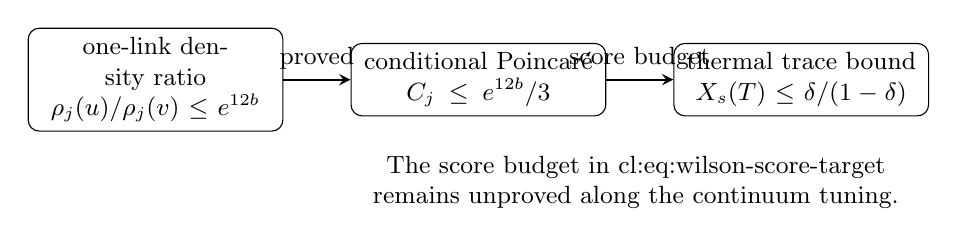
\begin{tikzpicture}[>=stealth,every node/.style={font=\small,align=center}]
\node[draw,rounded corners,text width=3cm] (a) at (0,0)
{one-link density ratio\\$\rho_j(u)/\rho_j(v)\le e^{12b}$};
\node[draw,rounded corners,text width=3cm] (b) at (4.1,0)
{conditional Poincar\'e\\$C_j\le e^{12b}/3$};
\node[draw,rounded corners,text width=3cm] (c) at (8.2,0)
{thermal trace bound\\$X_s(T)\le\delta/(1-\delta)$};
\draw[->,thick] (a)--node[above]{proved} (b);
\draw[->,thick] (b)--node[above]{score budget} (c);
\node[text width=7cm] at (6.1,-1.3)
{The score budget in \eqref{cl:eq:wilson-score-target} remains unproved
along the continuum tuning.};
\end{tikzpicture}
\caption{The conditional comparison is independent of volume and includes
all link fields. Its use in the cube criterion also requires decay of
the transition likelihood scores over a physical time interval.}
\label{cl:fig:fisher}
\end{figure}

The corollary separates two estimates. The conditional comparison has
been proved for every finite coupling. The time-dependent score budget
\eqref{cl:eq:wilson-score-target} has not. The factor $e^{12b}$ grows
along weak-coupling tuning; it cannot be hidden in a cutoff-independent
constant. Even a fixed physical cube has $3V(s)=24T^3$ revealed links,
so a bound on each score that is merely uniform in $j$ is insufficient.
A block ordering with a better conditional constant, a genuinely
time-decaying score bound or direct cancellation in the signed response
\eqref{cl:eq:replica-covariance} would require further estimates.

\subsection{The accuracy required of a free-energy remainder}
The leading weak-coupling free energy is a bulk quantity. Recent explicit
evaluation of its Maxwell constant \cite{Bre26} does not by itself
control the thermal defect. To quantify the distinction, fix the same
spatial torus and coupling and suppose
\[
\log Z(s,T)=VTf(b)+r_T,\qquad
\log Z(s,2T)=2VTf(b)+r_{2T}.
\]
The cancellation is exact: $\psi_s(T)=2r_T-r_{2T}$. Separate estimates
$|r_T|\le\varepsilon VT$ and $|r_{2T}|\le2\varepsilon VT$ give only
\[
\psi_{(2T)^3}(T)\le4\varepsilon VT=32\varepsilon T^4.
\]
Thus this method would require $\varepsilon\le1/(131104T^4)$ to prove
\Mcirc{}. A remainder stated only as $o(1)$ in the free-energy density
has no such rate. These error assumptions concern the periodic boxes
actually used here; asymptotics with other boundary conditions need an
additional boundary comparison. Likewise the weak-coupling decay theorem
for finite gauge groups \cite{AC25} supplies no uniform estimate for
continuous $\SU(2)$ merely by replacing the group in its statement.
